%% 8.1 %%

\setcounter{section}{0}
\section{The Generalized Riemann Integral}
\setcounter{exercise}{0}

\bx{
\ea{
\item The Riemann sum $R(f, P)$
chooses tags that are in between the $\inf, \sup$ of every interval,
so it must be between $L, U$.

We know $\int_a^b f = U = L$, so it is $\geq L(f, P)$ and $\leq U(f, P)$.

\item We chose $P_\epsilon$ such that $U(f, P_\epsilon) - L(f, P_\epsilon) < \epsilon/3$,
and $P'$ contains more points than $P_\epsilon$, so the difference can only be smaller.
}
}

\bx{
$P \subseteq P'$, so as we saw in Chapter 7, adding more points 
to the partition gives us more opportunities to have a smaller $\sup$
in every interval, so we conclude 
\begin{equation*}
  U(f, P) - U(f, P') \geq 0
\end{equation*}
}

\bx{
\ea{
\item The intervals that will be different will be when $P_\epsilon$
contributes a point between an interval of $P$, where it will break into two segments
that are different from the original. This produces a total of 3 segments that are 
potentially different. Since $P_\epsilon$ has $n+1$ points, 2 of the points are 
for the endpoints, so we can have $n-1$ of these 3 segment differences, i.e.
a total of $3(n-1)$ differences

\item We have $3(n-1)$ segment differences, and each segment is bounded by contribution 
\begin{equation*}
  \abs{
    M \cdot \delta
  }
\end{equation*}
since we chose $\delta$-fine segments.

Thus, we can show 
\begin{equation*}
  U(f, P) - U(f, P') \leq
  3(n-1) \cdot \delta \cdot M 
  <
  \frac{\epsilon}{9nM} \cdot 3(n-1) \cdot M
  < \epsilon/3
\end{equation*}
}

The proof finishes by showing a similar result for the other side,
and then we can conclude that 
$R(f, P), \int_a^b f$ are sandwiched between $L(f, P), U(f, P)$,
which in turn are sandwiched between $L(f, P')-\epsilon/3, U(f, P')+\epsilon/3$,
and $L(f, P'), U(f, P')$ themselves are $<\epsilon/3$ apart, so 
in all, $L(f, P), U(f, P)$ are sandwiched in an interval of length $\epsilon$,
so we conclude $R(f, P), \int_a^b f$ are also $< \epsilon$ apart.
}

\bx{
\ea{
\item 
We want to say we can just pick $c_k = \sup_x [x_k, x_{k+1}]$,
but the issue is $\sup$ might not exist in this interval;
imagine approaching $f(x) = 3$ infinitely closely, but never
getting there. Then we know $\sup f = 3$, but $\not\exists x' f(x') = 3$
in this interval.

If we have $f$ continuous, then $\sup$ (and $\inf$) exists,
so we can choose these $c_k$ to make $R(f, P) = U(f, P)$.

\item If $f$ is not continuous, we still know $f$ is bounded,
so no matter what $\sup f$ is on an interval, we can always get arbitrarily
close to it.

Then, all we have to do is make sure that 
\begin{equation*}
  \abs{
    \sup f_k - f(c_k)
  } < \epsilon_1
\end{equation*}
is small enough such that when we add all the intervals together, 
it is still $< \epsilon$.

We can choose $\epsilon_1 < \frac{\epsilon}{b-a}$
to do that.
}
\label{chap8:ex:partition_tagging}
}

\bx{
We showed in Exercise
\ref{chap8:ex:partition_tagging}
that 
\begin{align*}
  U(f, P) - R(f, P^1) &< \epsilon\\
  R(f, P^2) - L(f, P) &< \epsilon
\end{align*}
Where $P^1, P^2$ are different taggings of $P$.

Now, if we add these two questions together, we get 
\begin{equation*}
  U(f, P) - L(f, P) < 2\epsilon + \pbra{
    R(f, P^1) - R(f, P^2)
  }
\end{equation*}
So if we could bound the difference between the tagged partitions, 
we can finish our proof.

Fortunately, in this direction, we know that for some $\delta$-fine 
$P$, it is possible to show that for \textit{any} tagging of $P$,
we have 
\begin{equation*}
  \abs{
    R(f, P) - A
  } < \epsilon 
  \Rightarrow \abs{
    R(f, P^1) - R(f, P^2)
  } < \epsilon
\end{equation*}

Therefore, we can do the following, 
\begin{enumerate}[label=\arabic*.]
  \item Choose $\delta$ so that 
  \begin{equation*}
    \abs{
      R(f, P) - A
    } < \frac{\epsilon}{4}
    \Rightarrow \abs{
      R(f, P^j) - R(f, P^k)
    } < \frac{\epsilon}{4}
  \end{equation*}

  \item Choose partitions $P^1, P^2$ so that we have 
  \begin{align*}
    U(f, P) - R(f, P^1) &< \frac{\epsilon}{4}\\
    R(f, P^2) - L(f, P) &< \frac{\epsilon}{4}
  \end{align*}

  so we can say 
  \begin{equation*}
    U(f, P) - L(f, P) < \frac{\epsilon}{2} + \pbra{
      R(f, P^1) - R(f, P^2)
    } < \epsilon
  \end{equation*}
\end{enumerate}
Therefore, we can conclude $f$ is integrable.

To show that $\int_a^b f = A$, see that 
$R(f, P^1)$ is $\epsilon/4$ away from $A$, and 
$U(f, P)$ is $\epsilon/4$ away from $R(f, P^1)$,
so therefore $U(f, P)$ is $\epsilon/2$ away from $A$.
We also see that $L(f, P)$ is $\epsilon/2$ away from $A$
as well, so therefore we know $U(f) = \int_a^b f$,
is close to $A$
\begin{equation*}
  \abs{
    \int_a^b f - A
  } < \epsilon
\end{equation*}
}

\bx{
\ea{
\item We just need $x_k - x_{k-1} < \delta(c_k) = 1/9$, 
so any partition with intervals width $< 1/9$ will do.

\item We can choose the partition 
\begin{equation*}
  P = \pbrac{
    0, 
    1/4,
    1/4 + 1/12,
    1/4 + 2/12,
    \dots,
    1/4 + 8/12,
    1
  }
\end{equation*}
and choose tags as the left endpoint of the first interval,
and the right endpoint of the rest.

The reason this works is in the initial interval has tag $1/4$ and
size $1/4$. For every subsequent interval, the minimum 
tag has $>1/12$, so as long as we make the interval smaller than that,
we are fine.

\begin{figure}[H]
  \centering
  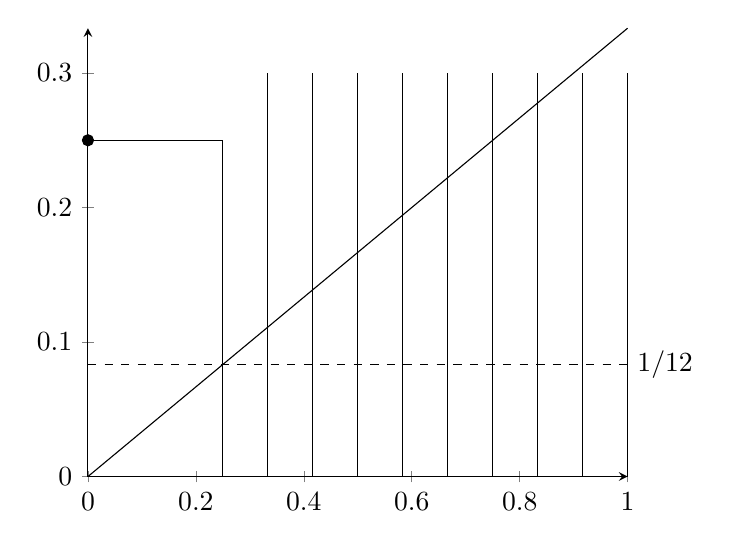
\begin{tikzpicture}
    \begin{axis}[
      axis y line=left,
      axis x line=bottom,
      clip = false
    ]
      \addplot[
        domain=0:1,
        samples=10
      ]{
        x/3
      };

      \addplot[mark=*] coordinates {
        (0, 1/4)
      };

      % Choosing partition
      \draw 
        (axis cs:1/4, 0) -- (axis cs:1/4, 1/4) -- 
        (axis cs:0, 1/4)
        (axis cs:1/4+1/12, 0) -- (axis cs:1/4+1/12, 0.3)
        (axis cs:1/4+2/12, 0) -- (axis cs:1/4+2/12, 0.3)
        (axis cs:1/4+3/12, 0) -- (axis cs:1/4+3/12, 0.3)
        (axis cs:1/4+4/12, 0) -- (axis cs:1/4+4/12, 0.3)
        (axis cs:1/4+5/12, 0) -- (axis cs:1/4+5/12, 0.3)
        (axis cs:1/4+6/12, 0) -- (axis cs:1/4+6/12, 0.3)
        (axis cs:1/4+7/12, 0) -- (axis cs:1/4+7/12, 0.3)
        (axis cs:1/4+8/12, 0) -- (axis cs:1/4+8/12, 0.3)
        (axis cs:1, 0) -- (axis cs:1, 0.3)
        (axis cs:1/4+1/12, 0) -- (axis cs:1/4+1/12, 0.3)
      ;

      \draw[dashed]
        (axis cs:0, 1/12) -- (axis cs:1, 1/12) node[right] {$1/12$}
      ;
    \end{axis}
  \end{tikzpicture}
  \caption{Choosing a $\delta(x)$-fine partition}
  \label{chap8:fig:choosing_delta_fine}
\end{figure}
}
}

\bx{
The intuition here is that eventually,
the partitions are so small that it must be $< \delta(x)$ for 
some $x$ in the interval.

\AFSOC this bisecting never ends.
Then by the NIP, we can find an $x$ that exists in the never-ending 
bisected intervals.
From our hypothesis, we know that for this $x$, every
\begin{equation*}
  \abs{I_n} > \delta(x)
\end{equation*}
However, since $\delta(x)$ is fixed here,
and we can find an arbitrarily small interval size,
this implies $\delta(x) = 0$, but this is a contradiction since $\delta(x) > 0$.

Therefore, we conclude that there must be a finite number of bisections,
and when the bisecting stops, $\exists x$ such that $\delta(x) > x_k - x_{k-1}$.
}

\bx{
Define 
\begin{equation*}
  \delta(x) = 
  \min(\delta_1(x), \delta_2(x)),
\end{equation*}
then we can find some tagged partition $(P, \pbrac{c_k}_{k=1}^n)$
that is $\delta(x)$-fine.

Now, this tagged partition is also $\delta_1, \delta_2$-fine since 
in every interval,
\begin{equation*}
  x_k - x_{k-1} < \delta(c_k) = 
  \min(\delta_1(c_k), \delta_2(c_k)),
\end{equation*}
and therefore $x_k - x_{k-1}$ is smaller than both $\delta_1, \delta_2$.

Therefore $A_1, A_2$ are $\epsilon/2$ away from a common element,
which means we can show they are 
\begin{equation*}
  \abs{
    A_1 - A_2
  } < \epsilon
\end{equation*}
}

\bx{
If a function is Riemann Integrable, 
we know that it has a $\delta_0$ such that for any 
$\delta_0$-fine tagged partition we have 
\begin{equation*}
  \abs{
    R(f, P) - A
  } < \epsilon
\end{equation*}
We can choose $\delta(x) = \delta_0$ to satisfy the above
property, and therefore we have found a gauge that works
and shows $f$ is Generalized Riemann Integrable.
}

\bx{
If we have a tagged partition that is $\delta(x)$-fine by 
our definition, we know that every interval containing
a rational number $r_k$ is width at most $\epsilon/2^{k+1}$.
Now, this $r_k$ could also be on the endpoint of an interval,
in which case it appears twice.

So in the worst case, we can calculate 
\begin{equation*}
  R(f, P) < \sum_{k=1}^\infty 2\cdot \frac{\epsilon}{2^{k+1}} \cdot \pa{\sup g(c_k)}
  = \sum_{k=1}^\infty \frac{\epsilon}{2^{k}} \cdot 1
  = \epsilon
\end{equation*}
}

\bx{
This is just a telescoping series, with the endpoints $a, b$.
}

\bx{
We know $F'(c) = f(c)$, so we must have some $V_\delta(c)$
such that for any $x$ in this neighborhood, 
the derivative is $\epsilon$ close to $f(c)$.

Then, we can define the gauage to be this $\delta$ for every $c$.
\label{chap8:ex:close_derivative}
}

\bx{
\ea{
\item Both of these results follow from Exercise
\ref{chap8:ex:close_derivative},
since our $P$ is $\delta(c)$-fine, so any 
$c$ chosen in the $[x_{k-1}, x_k]$ interval is 
$\delta(c)$ close to either endpoint.

\item We can add up 
\begin{align*}
  -\epsilon(x_k - c_k) &< F(x_k) - F(c_k) - f(c_k)(x_k-c_k) < \epsilon(x_k-c_k)\\
  -\epsilon(c_k - x_{k-1}) &< F(c_k) - F(x_{k-1}) - f(c_k)(c_k-x_{k-1}) < \epsilon(c_k-x_{k-1})\\
  -\epsilon(x_k - x_{k-1}) &< F(x_k) - F(x_{k-1}) - f(c_k)(x_k-x_{k-1}) < \epsilon(x_k-x_{k-1})\\
  \Rightarrow &\abs{
    F(x_k) - F(x_{k-1}) - f(c_k)(x_k-x_{k-1})
  } < \epsilon(x_k - x_{k-1})
\end{align*}
}

From here, we know that our difference 
\begin{equation*}
  \abs{
    F(b) - F(a) - R(f, P)
  } < \epsilon'
\end{equation*}
}

\bx{
\ea{
\item We just need to show that 
\begin{equation*}
  \pa{
    F(g(x))
  }' = F'(g(x)) \cdot g'(x)
\end{equation*}
exists, but this is true since we said $g$ is differentiable on $[a, b]$
and $F$ is differentiable on the set $g([a, b])$.

\item We can show 
\begin{align*}
  F(g(b)) - F(g(a)) 
  &= 
  \int_a^b \pa{
    F(g(x))
  }' \dd{x} \\
  &= 
  \int_a^b F'(g(x)) \cdot g'(x) \dd{x}\\
  &=
  \int_a^b f(g(x)) \cdot g'(x) \dd{x}
\end{align*}

\item Since $F$ is differentiable at each point $g([a, b])$,
we can directly apply Theorem 8.1.9 and conclude that 
\begin{equation*}
  \int_{g(a))}^{g(b)} f = F(g(b)) - F(g(a))
\end{equation*}
}
}